
%% bare_conf.tex
%% V1.3
%% 2007/01/11
%% by Michael Shell
%% See:
%% http://www.michaelshell.org/
%% for current contact information.
%%
%% This is a skeleton file demonstrating the use of IEEEtran.cls
%% (requires IEEEtran.cls version 1.7 or later) with an IEEE conference paper.
%%
%% Support sites:
%% http://www.michaelshell.org/tex/ieeetran/
%% http://www.ctan.org/tex-archive/macros/latex/contrib/IEEEtran/
%% and
%% http://www.ieee.org/

%%*************************************************************************
%% Legal Notice:
%% This code is offered as-is without any warranty either expressed or
%% implied; without even the implied warranty of MERCHANTABILITY or
%% FITNESS FOR A PARTICULAR PURPOSE! 
%% User assumes all risk.
%% In no event shall IEEE or any contributor to this code be liable for
%% any damages or losses, including, but not limited to, incidental,
%% consequential, or any other damages, resulting from the use or misuse
%% of any information contained here.
%%
%% All comments are the opinions of their respective authors and are not
%% necessarily endorsed by the IEEE.
%%
%% This work is distributed under the LaTeX Project Public License (LPPL)
%% ( http://www.latex-project.org/ ) version 1.3, and may be freely used,
%% distributed and modified. A copy of the LPPL, version 1.3, is included
%% in the base LaTeX documentation of all distributions of LaTeX released
%% 2003/12/01 or later.
%% Retain all contribution notices and credits.
%% ** Modified files should be clearly indicated as such, including  **
%% ** renaming them and changing author support contact information. **
%%
%% File list of work: IEEEtran.cls, IEEEtran_HOWTO.pdf, bare_adv.tex,
%%                    bare_conf.tex, bare_jrnl.tex, bare_jrnl_compsoc.tex
%%*************************************************************************

% *** Authors should verify (and, if needed, correct) their LaTeX system  ***
% *** with the testflow diagnostic prior to trusting their LaTeX platform ***
% *** with production work. IEEE's font choices can trigger bugs that do  ***
% *** not appear when using other class files.                            ***
% The testflow support page is at:
% http://www.michaelshell.org/tex/testflow/



% Note that the a4paper option is mainly intended so that authors in
% countries using A4 can easily print to A4 and see how their papers will
% look in print - the typesetting of the document will not typically be
% affected with changes in paper size (but the bottom and side margins will).
% Use the testflow package mentioned above to verify correct handling of
% both paper sizes by the user's LaTeX system.
%
% Also note that the "draftcls" or "draftclsnofoot", not "draft", option
% should be used if it is desired that the figures are to be displayed in
% draft mode.
%
\documentclass[conference]{IEEEtran}
% Add the compsoc option for Computer Society conferences.
%
% If IEEEtran.cls has not been installed into the LaTeX system files,
% manually specify the path to it like:
% \documentclass[conference]{../sty/IEEEtran}





% Some very useful LaTeX packages include:
% (uncomment the ones you want to load)


% *** MISC UTILITY PACKAGES ***
%
%\usepackage{ifpdf}
% Heiko Oberdiek's ifpdf.sty is very useful if you need conditional
% compilation based on whether the output is pdf or dvi.
% usage:
% \ifpdf
%   % pdf code
% \else
%   % dvi code
% \fi
% The latest version of ifpdf.sty can be obtained from:
% http://www.ctan.org/tex-archive/macros/latex/contrib/oberdiek/
% Also, note that IEEEtran.cls V1.7 and later provides a builtin
% \ifCLASSINFOpdf conditional that works the same way.
% When switching from latex to pdflatex and vice-versa, the compiler may
% have to be run twice to clear warning/error messages.






% *** CITATION PACKAGES ***
%
%\usepackage{cite}
% cite.sty was written by Donald Arseneau
% V1.6 and later of IEEEtran pre-defines the format of the cite.sty package
% \cite{} output to follow that of IEEE. Loading the cite package will
% result in citation numbers being automatically sorted and properly
% "compressed/ranged". e.g., [1], [9], [2], [7], [5], [6] without using
% cite.sty will become [1], [2], [5]--[7], [9] using cite.sty. cite.sty's
% \cite will automatically add leading space, if needed. Use cite.sty's
% noadjust option (cite.sty V3.8 and later) if you want to turn this off.
% cite.sty is already installed on most LaTeX systems. Be sure and use
% version 4.0 (2003-05-27) and later if using hyperref.sty. cite.sty does
% not currently provide for hyperlinked citations.
% The latest version can be obtained at:
% http://www.ctan.org/tex-archive/macros/latex/contrib/cite/
% The documentation is contained in the cite.sty file itself.






% *** GRAPHICS RELATED PACKAGES ***
%
\ifCLASSINFOpdf
  \usepackage[pdftex]{graphicx}
  % declare the path(s) where your graphic files are
  \graphicspath{{./images/}}
  % and their extensions so you won't have to specify these with
  % every instance of \includegraphics
  \DeclareGraphicsExtensions{.jpg}
\else
  % or other class option (dvipsone, dvipdf, if not using dvips). graphicx
  % will default to the driver specified in the system graphics.cfg if no
  % driver is specified.
  \usepackage[dvips]{graphicx}
  % declare the path(s) where your graphic files are
  \graphicspath{{./images/}}
  % and their extensions so you won't have to specify these with
  % every instance of \includegraphics
  \DeclareGraphicsExtensions{.eps}
\fi
% graphicx was written by David Carlisle and Sebastian Rahtz. It is
% required if you want graphics, photos, etc. graphicx.sty is already
% installed on most LaTeX systems. The latest version and documentation can
% be obtained at: 
% http://www.ctan.org/tex-archive/macros/latex/required/graphics/
% Another good source of documentation is "Using Imported Graphics in
% LaTeX2e" by Keith Reckdahl which can be found as epslatex.ps or
% epslatex.pdf at: http://www.ctan.org/tex-archive/info/
%
% latex, and pdflatex in dvi mode, support graphics in encapsulated
% postscript (.eps) format. pdflatex in pdf mode supports graphics
% in .pdf, .jpeg, .png and .mps (metapost) formats. Users should ensure
% that all non-photo figures use a vector format (.eps, .pdf, .mps) and
% not a bitmapped formats (.jpeg, .png). IEEE frowns on bitmapped formats
% which can result in "jaggedy"/blurry rendering of lines and letters as
% well as large increases in file sizes.
%
% You can find documentation about the pdfTeX application at:
% http://www.tug.org/applications/pdftex





% *** MATH PACKAGES ***
%
%\usepackage[cmex10]{amsmath}
% A popular package from the American Mathematical Society that provides
% many useful and powerful commands for dealing with mathematics. If using
% it, be sure to load this package with the cmex10 option to ensure that
% only type 1 fonts will utilized at all point sizes. Without this option,
% it is possible that some math symbols, particularly those within
% footnotes, will be rendered in bitmap form which will result in a
% document that can not be IEEE Xplore compliant!
%
% Also, note that the amsmath package sets \interdisplaylinepenalty to 10000
% thus preventing page breaks from occurring within multiline equations. Use:
%\interdisplaylinepenalty=2500
% after loading amsmath to restore such page breaks as IEEEtran.cls normally
% does. amsmath.sty is already installed on most LaTeX systems. The latest
% version and documentation can be obtained at:
% http://www.ctan.org/tex-archive/macros/latex/required/amslatex/math/





% *** SPECIALIZED LIST PACKAGES ***
%
%\usepackage{algorithmic}
% algorithmic.sty was written by Peter Williams and Rogerio Brito.
% This package provides an algorithmic environment fo describing algorithms.
% You can use the algorithmic environment in-text or within a figure
% environment to provide for a floating algorithm. Do NOT use the algorithm
% floating environment provided by algorithm.sty (by the same authors) or
% algorithm2e.sty (by Christophe Fiorio) as IEEE does not use dedicated
% algorithm float types and packages that provide these will not provide
% correct IEEE style captions. The latest version and documentation of
% algorithmic.sty can be obtained at:
% http://www.ctan.org/tex-archive/macros/latex/contrib/algorithms/
% There is also a support site at:
% http://algorithms.berlios.de/index.html
% Also of interest may be the (relatively newer and more customizable)
% algorithmicx.sty package by Szasz Janos:
% http://www.ctan.org/tex-archive/macros/latex/contrib/algorithmicx/




% *** ALIGNMENT PACKAGES ***
%
%\usepackage{array}
% Frank Mittelbach's and David Carlisle's array.sty patches and improves
% the standard LaTeX2e array and tabular environments to provide better
% appearance and additional user controls. As the default LaTeX2e table
% generation code is lacking to the point of almost being broken with
% respect to the quality of the end results, all users are strongly
% advised to use an enhanced (at the very least that provided by array.sty)
% set of table tools. array.sty is already installed on most systems. The
% latest version and documentation can be obtained at:
% http://www.ctan.org/tex-archive/macros/latex/required/tools/


%\usepackage{mdwmath}
%\usepackage{mdwtab}
% Also highly recommended is Mark Wooding's extremely powerful MDW tools,
% especially mdwmath.sty and mdwtab.sty which are used to format equations
% and tables, respectively. The MDWtools set is already installed on most
% LaTeX systems. The lastest version and documentation is available at:
% http://www.ctan.org/tex-archive/macros/latex/contrib/mdwtools/


% IEEEtran contains the IEEEeqnarray family of commands that can be used to
% generate multiline equations as well as matrices, tables, etc., of high
% quality.


%\usepackage{eqparbox}
% Also of notable interest is Scott Pakin's eqparbox package for creating
% (automatically sized) equal width boxes - aka "natural width parboxes".
% Available at:
% http://www.ctan.org/tex-archive/macros/latex/contrib/eqparbox/





% *** SUBFIGURE PACKAGES ***
%\usepackage[tight,footnotesize]{subfigure}
% subfigure.sty was written by Steven Douglas Cochran. This package makes it
% easy to put subfigures in your figures. e.g., "Figure 1a and 1b". For IEEE
% work, it is a good idea to load it with the tight package option to reduce
% the amount of white space around the subfigures. subfigure.sty is already
% installed on most LaTeX systems. The latest version and documentation can
% be obtained at:
% http://www.ctan.org/tex-archive/obsolete/macros/latex/contrib/subfigure/
% subfigure.sty has been superceeded by subfig.sty.



%\usepackage[caption=false]{caption}
%\usepackage[font=footnotesize]{subfig}
% subfig.sty, also written by Steven Douglas Cochran, is the modern
% replacement for subfigure.sty. However, subfig.sty requires and
% automatically loads Axel Sommerfeldt's caption.sty which will override
% IEEEtran.cls handling of captions and this will result in nonIEEE style
% figure/table captions. To prevent this problem, be sure and preload
% caption.sty with its "caption=false" package option. This is will preserve
% IEEEtran.cls handing of captions. Version 1.3 (2005/06/28) and later 
% (recommended due to many improvements over 1.2) of subfig.sty supports
% the caption=false option directly:
%\usepackage[caption=false,font=footnotesize]{subfig}
%
% The latest version and documentation can be obtained at:
% http://www.ctan.org/tex-archive/macros/latex/contrib/subfig/
% The latest version and documentation of caption.sty can be obtained at:
% http://www.ctan.org/tex-archive/macros/latex/contrib/caption/




% *** FLOAT PACKAGES ***
%
%\usepackage{fixltx2e}
% fixltx2e, the successor to the earlier fix2col.sty, was written by
% Frank Mittelbach and David Carlisle. This package corrects a few problems
% in the LaTeX2e kernel, the most notable of which is that in current
% LaTeX2e releases, the ordering of single and double column floats is not
% guaranteed to be preserved. Thus, an unpatched LaTeX2e can allow a
% single column figure to be placed prior to an earlier double column
% figure. The latest version and documentation can be found at:
% http://www.ctan.org/tex-archive/macros/latex/base/



%\usepackage{stfloats}
% stfloats.sty was written by Sigitas Tolusis. This package gives LaTeX2e
% the ability to do double column floats at the bottom of the page as well
% as the top. (e.g., "\begin{figure*}[!b]" is not normally possible in
% LaTeX2e). It also provides a command:
%\fnbelowfloat
% to enable the placement of footnotes below bottom floats (the standard
% LaTeX2e kernel puts them above bottom floats). This is an invasive package
% which rewrites many portions of the LaTeX2e float routines. It may not work
% with other packages that modify the LaTeX2e float routines. The latest
% version and documentation can be obtained at:
% http://www.ctan.org/tex-archive/macros/latex/contrib/sttools/
% Documentation is contained in the stfloats.sty comments as well as in the
% presfull.pdf file. Do not use the stfloats baselinefloat ability as IEEE
% does not allow \baselineskip to stretch. Authors submitting work to the
% IEEE should note that IEEE rarely uses double column equations and
% that authors should try to avoid such use. Do not be tempted to use the
% cuted.sty or midfloat.sty packages (also by Sigitas Tolusis) as IEEE does
% not format its papers in such ways.





% *** PDF, URL AND HYPERLINK PACKAGES ***
%
%\usepackage{url}
% url.sty was written by Donald Arseneau. It provides better support for
% handling and breaking URLs. url.sty is already installed on most LaTeX
% systems. The latest version can be obtained at:
% http://www.ctan.org/tex-archive/macros/latex/contrib/misc/
% Read the url.sty source comments for usage information. Basically,
% \url{my_url_here}.





% *** Do not adjust lengths that control margins, column widths, etc. ***
% *** Do not use packages that alter fonts (such as pslatex).         ***
% There should be no need to do such things with IEEEtran.cls V1.6 and later.
% (Unless specifically asked to do so by the journal or conference you plan
% to submit to, of course. )


% correct bad hyphenation here
%\hyphenation{op-tical net-works semi-conduc-tor}

\usepackage{tikz}
\usetikzlibrary{arrows}

\usepackage{amsmath}

%\usepackage{natbib}

\begin{document}
%
% paper title
% can use linebreaks \\ within to get better formatting as desired
\title{Graphical formalization and automated computing of safety constraints in robotics}


% author names and affiliations
% use a multiple column layout for up to three different
% affiliations
\author{\IEEEauthorblockN{Ludwig N\"{a}gele}
\IEEEauthorblockA{Department of Software Engineering and\\Programming Languages\\ 
University of Augsburg\\
86135 Augsburg, Germany\\
Email: mail@ludwig-naegele.de}
\and
\IEEEauthorblockN{Bruce A. MacDonald}
\IEEEauthorblockA{Department of Electrical Engineering\\ 
The University of Auckland\\
Auckland 1142, New Zealand\\
Email: b.macdonald@auckland.ac.nz}
%\and
%\IEEEauthorblockN{James Kirk\\ and Montgomery Scott}
%\IEEEauthorblockA{Starfleet Academy\\
%San Francisco, California 96678-2391\\
%Telephone: (800) 555--1212\\
%Fax: (888) 555--1212}
}

% conference papers do not typically use \thanks and this command
% is locked out in conference mode. If really needed, such as for
% the acknowledgment of grants, issue a \IEEEoverridecommandlockouts
% after \documentclass

% for over three affiliations, or if they all won't fit within the width
% of the page, use this alternative format:
% 
%\author{\IEEEauthorblockN{Michael Shell\IEEEauthorrefmark{1},
%Homer Simpson\IEEEauthorrefmark{2},
%James Kirk\IEEEauthorrefmark{3}, 
%Montgomery Scott\IEEEauthorrefmark{3} and
%Eldon Tyrell\IEEEauthorrefmark{4}}
%\IEEEauthorblockA{\IEEEauthorrefmark{1}School of Electrical and Computer Engineering\\
%Georgia Institute of Technology,
%Atlanta, Georgia 30332--0250\\ Email: see http://www.michaelshell.org/contact.html}
%\IEEEauthorblockA{\IEEEauthorrefmark{2}Twentieth Century Fox, Springfield, USA\\
%Email: homer@thesimpsons.com}
%\IEEEauthorblockA{\IEEEauthorrefmark{3}Starfleet Academy, San Francisco, California 96678-2391\\
%Telephone: (800) 555--1212, Fax: (888) 555--1212}
%\IEEEauthorblockA{\IEEEauthorrefmark{4}Tyrell Inc., 123 Replicant Street, Los Angeles, California 90210--4321}}




% use for special paper notices
%\IEEEspecialpapernotice{(Invited Paper)}




% make the title area
\maketitle


\begin{abstract}
%\boldmath
Nowadays robotic applications are no longer confined to only industrial use but increasingly assigned to jobs within human workspaces. Even the programming of robots is shifting from experienced software developers to the consumers themselves who need to customize the robot's behavior in order to match the user's individual tasks and requirements.
However both the human robot collaboration as well as the behavior definition by non experts may be a risk to humans within the robots' environment.
Thus special thinking is needed about how to cope with safety requirements for robot behavior specification by consumers.
%about how safety could be achieved in this scope.

%to make human robot interaction safe and espacially how to make user defined behavior safe.
%Special highlevel tools are developed in order to allow behavior definition by non experts.
%Besides the fact that human robot collaboration is becoming highly important, it has also to be thought about convenient safety mechanisms. 

In this paper we present a visual language for the defining of safety constraints for state machine definition of robot behaviour. Our approach addresses mainly non-safety-experts and our abstraction from a mathematical temporal logic expression to a more intuitive visual representation is intended to enable a wider range of software developers to do model checking.
Furthermore we propose a new concept of development support %and qualit�tssicherung
by providing automated constraint generation functionality. It aims to help developers in defining reasonable constraints and finally to increase the probability of finding bugs.

A graphical editor has been developed which demonstrates both visual constraint creation functionality as well as automated constraint generation. 

%Our purpose is to target non experts and to make safety checking available for a bigger community. Hence we had a special focus on a simple syntax and easy understandability as well as active support  in our approach.

%Among others robots are alredy used in elderly care centers for healthcare purpose.

\end{abstract}
% IEEEtran.cls defaults to using nonbold math in the Abstract.
% This preserves the distinction between vectors and scalars. However,
% if the conference you are submitting to favors bold math in the abstract,
% then you can use LaTeX's standard command \boldmath at the very start
% of the abstract to achieve this. Many IEEE journals/conferences frown on
% math in the abstract anyway.

% no keywords




% For peer review papers, you can put extra information on the cover
% page as needed:
% \ifCLASSOPTIONpeerreview
% \begin{center} \bfseries EDICS Category: 3-BBND \end{center}
% \fi
%
% For peerreview papers, this IEEEtran command inserts a page break and
% creates the second title. It will be ignored for other modes.
\IEEEpeerreviewmaketitle











%----------------------------------------------------------------------
% SECTION I: Introduction
%----------------------------------------------------------------------
\section{Introduction}

%\IEEEPARstart{S}{afety}
Safety critical applications require extensive testing or formal verification in order to achieve adequate safe and predictable behavior.
Even if a more highlevel program has no physical movements and thus cannot directly cause any damage, its output might still be a trigger for dangerous actions executed by interacting actors.
%Even if a more highlevel program has no physical actors and thus cannot cause any damage, it might still have dangerous effects on the environment.
Imagine a medication reminder application which guides a person through the process of medication intake, such as the healthcare robotics project at the University of Auckland, New Zealand \cite{jayawardena12:_desig}. All interaction is by showing textual instructions on a display, and by speech generation. An error in the program logic could cause an already taken medication to be reminded again and may injure a patient with Alzheimer's disease by causing a medication overdose.
Scientists are working on applications such as the medication reminder~\cite{p11:_feasib} which run on mobile robots serving in nursing homes for the elderly. Equipped with a touch display and several external devices such as a blood pressure measurement tool the robots aim to support and entertain the elderly in their daily activities~\cite{jayawardena12:_desig,5649910}.
The applications are intended to be developed by healthcare professionals using Robostudio~\cite{robostudio}, a visual programming environment for rapid authoring and customization of complex services on a personal service robot.
%state machine based processes and a graphical tool for the designing of human robot interaction.
Generally these people don't have profound knowledge of the complex mathematical syntax used for formal verification methods such as computation tree logic (CTL) or linear temporal logic (LTL). Nevertheless certain safety guarantees must somehow be delivered in order to gain users' trust and to prevent any harm or injuries by the healthcare robots.
In case of the medication reminder mentioned above it might be important to ensure notifications are sent to staff members whenever medication is not taken by the patient, or to avoid duplicate reminders for medications which have already been taken.

So a mechanism is needed for the specification of such safety constraints; one that does not require special or expert knowledge and thus is easy to use for all kind of programmers. A visual language intended to fill this gap is presented in section~\ref{sec:visualformalism}.

Unfortunately the supply of an easy-to-use editor for constraint creation doesn't guarantee adequate thinking about sufficent constraints by the developer. Unmotivated or just unexperienced developers may miss important constraints needed in order to achieve a certain safety level.
To support the user in finding significant constraints it might be useful to automatically compute constraint suggestions which make true testimonies about the current designed program. First of all the generated constraints provide an opportunity for the developer to identify reasonable constraints as well as contradictions between constraints and specification. The latter would mean there are errors in the program which lead to undesired constraints. Furthermore once constraints are created and checked for sanity they can be validated after every program change and thus ensure integrity during the development process.

In section~\ref{sec:automatedconstraintgeneration} we introduce an heuristic for finding reasonable safety constraints based on a state machine in the healthcare robotics domain.

%Once such constraints are defined, they determine the grade of safety coverage. Unfortunately, the program may still contain errors if there is at least one significant constraint missed out. To support the user in finding such ones the tool could furthermore automatically compute suggestions for possible constraints based on the designed statemachine. These are displayed to the programmer and may help him identifying reasonable constraints as well as contradictions between program and specification.

%Our approach presented in this paper has a special focus on the healtcare domain.


%Dieses beispiel ist eine Anwendung eines umfangreichen Healthcare-Projekts, an dem im robotics lab der Universit�t von Auckland gearbeitet wird. Die zustansbasierten Anwendungen laufen auf Cafero, einem mit blutdruckmessger�t und anderen tools austestatteten mobilen Roboter mit Touchdisplay.
%Die einzelnen Anwendungen werden von Healthcare-Professionals mit dem Tool Robostudio [cite] entwickelt, das eine graphische oberfl�sche zur modellierung von zustandsmaschinen externen services und  bietet.
%Allerdings haben diese not to have profound knowledge of the complex mathematical syntax used for formal verification methods such as computation tree logic (CTL) or linear temporal logic (LTL)).
%Dennoch m�chte man gegen�ber den Patienten, die von solchen Robotern gepflegt werden, ein gewisses Level an Sicherheit gew�hrleisten k�nnen. Beispielsweise soll in obigem Beispiel sichergestellt werden k�nnen, dass ein Medikament nach der Einnahme nicht erneut in einer Erinnerung auftaucht, oder dass bei Nichteinnahme ein Mitarbeiter benachrichtigt wird.
%Dazu bedarf es allerdings Mechanismen zur spezifizierung solcher Sicherheitseigenschaften, die f�r den Programmentwickler zug�nglich und einfach (am besten ohne spezialwissen) zu benutzen sind.

%Constraints can be easily defined graphically and provide the user with an instant result about validity.
%, which can make propositions about the behavior of state machines.
%This language is an abstraction layer above temporal logic and allows a rather intuitive than textual model checking.
%The abstraction from textual and mathematical temporal logic expression allows a rather intuitive way of model checking and thus makes this language accessible to non-experts.

%CTL and LTL are important concepts for model checking and verification of statemachines. But their powerfulness is reflected in the complexity of their mathematical expressions, what makes it difficult to use for programmers who haven't got deeper expertise in this subject.

%The challenge now is to find a similar intuitive and nonmathematical way of representing reasonable safety constraints for the healthbot domain and to figure out how to translate it to corresponding textual expressions. The new concept will be integrated into Robostudio, a design tool for statemachines, in order to enable the user to create safety constraints visually. A common LTL model checker will be added to it as well which fulfils the verification of the translated constraints on the designed statemachine. In case of verification failures the concerning constraints and a visual counter example can be presented.

%Once such constraints are defined, they determine the grade of safety coverage. Unfortunately, the program may still contain errors if there is at least one significant constraint missed out. To support the user in finding such ones the tool could furthermore automatically compute suggestions for possible constraints based on the designed statemachine. These are displayed to the programmer and may help him identifying reasonable constraints as well as contradictions between program and specification.


%----------------------------------------------------------------------
% SECTION I: Introduction
%----------------------------------------------------------------------
\section{Related work}



%Was gibt es schon alles?

% 1993 A Visual-Programming Environment for a Temporal Logic Language
% 1995 Visual Specification of Branching Time Temporal Logic
% 2007 HomeTL: A visual formalism, based on temporal logic, for the design of home based care
% 2007 A Visual Editor to Support the Use of Temporal Logic for ADL Monitoring


A first step towards a graphical tool for the designing of safety constraints is taken by Sisiruca and Ionescu~\cite{332301}. They developed an object-oriented graphical environment for visually creating temporal logic sentences and rules. The tool presents temporal operators as logical modules with boolean inputs and outputs which can be connected to one big expression graph.

Also Del Bimbo {\em et al} worked on a visual tool for temporal logic, but with a special focus on hierarchical representations of formulas~\cite{520786}. Here each node of a tree is described by an abstract operator whose subformulas are branches to their replacement operators. Thus the root node represents the entire formula. They also explored the formula trees' 3D representation within a virtual space.

Both approaches are different fundamental ideas of representing temporal formulas. Whereas having a graph and inputs and outputs seems not to be applicable for our approach, the idea of hirarchical operator representation of Del Bimbo {\em et al} will be a good basis for our concept of constraint creation and understanding.

%aim for simplifying the development of constraints, but they still demand knowledge of the underlying mathematical formalism of temporal logic.

The step towards a more abstract level of development is taken by HomeTL~\cite{4341725}, a visual formalism for the design of home based care. It allows healthcare professionals to specify rules and sequences of user actions in a quite nontechnical manner. Based on these conditions a monitoring system in a patient's home environment can detect and report abnormal situations within the daily routine.

Even though this approach touches the subject of healthcare it barely matches our problem. HomeTL focuses more on monitoring temporal boundaries of a patient's behavior than on ensuring functional safety of an implemented program. It does depict how nontechnical constraint design can be realised and its graphical design is a good example of handling time dependencies.

%There are already works about constraint generation such as one approach of NASA [4], for example. They used test oracles in order to achieve consistency between program code and specification during development. 
% Das wollen wir auch erzielen mit unseren automatisch generierten constraints...

%But these kind of oracles are for automated test purpose and are rather complex than intuitive. However, our goal is to find nonmathematical and just intuitive ones. An intelligent heuristic must determine key states and possible conjunctions of them in order to build reasonable constraints. Afterwards they get filtered by an algorithm which computes importances for each constraint based on state weights. Finally the developer obtains a set of visual constraints which he can then check for plausibility.



%----------------------------------------------------------------------
% SECTION II: Requirements
%----------------------------------------------------------------------
\section{Requirements}
\label{sec:requirements}

% soll hier noch gesagt werden, dass wir davon ausgehen, dass es keine endzust�nde gibt?

We want to introduce a visual language for defining safety constraints in state machine definitions of robot behaviour, that is suitable for people who are not experts in formal methods. The visual language should be easy to use and intuitive to read, in order to facilitate maintainability.
Hence, the graphical formalism should abstract from the usually complex and mathematical concept of conventional formal methods but still be unreduced in expressiveness compared to LTL, so far as possible.
 
Furthermore a heuristic should be developed, which identifies reasonable constraints on an underlying state machine program. 
Since the particular domain semantics distinguish the significance of constraints, it may be difficult to show a universal heuristic. Hence, in this paper the concept of development support by constraint generation is examined within the domain of healthcare robotics. As a special requirement for the heuristic at least the following constraints are to be found for the medication reminder application:

\begin{itemize}
	\item The program will always eventually check the database for new reminder jobs. Thus we ensure that pending reminders are processed.
	\item Either a reminded medication is taken properly, or caregivers are notified that the patient refused medication intake.
% The next item is left out so that we can say, our heuristic found one we didn't think about yet :)
%	\item During the medication intake process the program can not switch to other services such as entertainment mode ore blood pressure measurement, for example.
\end{itemize}

Some of the statements do not make sense if patients lie or pretend to take their medication but don't take it. As our approach validates state machine behaviour rather than human attitudes we assume there is either cooperation from the patient or a separate tool that can verify medication intake. Furthermore we assume the correctness of external services used by the medication reminder such as the database module holding all reminders.

% Bruce: I'm not sure we need this sentence. I think you have integrated it now anyway.
% All the functionality mentioned above shall be combined in one editor and for evaluation purpose later be integrated into a programming environment for state machine editing.


%----------------------------------------------------------------------
% SECTION II: Design
%----------------------------------------------------------------------
\section{Design}

\subsection{Visual formalism}
\label{sec:visualformalism}

The presented visual language is designed to express constraints for state machines. To provide the required functionality, the fundamental logical operators are required, as shown in (a) though (e) below. In addition the visual language should be capable of expressing constraints about future steps, both (h) any future state and (g) the next state, that (f) events should always happen, and that (i) a property must be true until some future event.

 Like Del Bimbo {\em et al's} formula representation~\cite{520786}, a constraint consists of nested operators and propositions in a hierarchy. However we surrender the three dimensional idea and focus on two dimensional blocks and their compositions instead, what is also used by HomeTL~\cite{4341725}.
Each block represents either an operator or a proposition and has its specified semantics. Thus a visual formula can be recursively translated to a linear temporal logic (LTL) sentence and be checked using any ordinary model checker. 

The visual language has support for eight operator types and one proposition as shown in figure~\ref{fig:operators}. 

\begin{description}
	\item[(a)] \emph{AND} operator: $\varphi \wedge \psi$.
	\item[(b)] \emph{OR} Operator: $\varphi \vee \psi$.
	\item[(c)] \emph{IF} operator: $\varphi \Rightarrow \psi$.\\Instead of an \emph{IMPLIES} operator an \emph{IF} operator is provided. Its meaning seems to be more intuitive for non-experts since it is a common construct in almost every programming language.
	\item[(d)] \emph{NOT} operator: $\neg \varphi$.
	\item[(e)] Proposition: $\rho$.\\Until now there is only the \emph{state proposition} type, which gives evidence about the currently active state. Other types such as numeric or string equations may be added but are less important for our healthcare subject.
	\item[(f)] \emph{FUTURE} operator: $F \varphi$.\\At least one time -- now or in a later state -- $\varphi$ must be true.
	\item[(g)] \emph{ALWAYS} operator: $G \varphi$.\\$\varphi$ must be true now and in all following states.
	\item[(h)] \emph{NEXT} operator: $X \varphi$.\\$\varphi$ has to be true in the next state.
	\item[(i)] \emph{UNTIL} operator: $[\varphi U \psi]$.\\Now and in all following states $\varphi$ must be true until there is a state with $\psi$ being true. In addition eventually there has to be a future state with $\psi$ being true.
\end{description}


\begin{figure}[htbp]
  \centering
  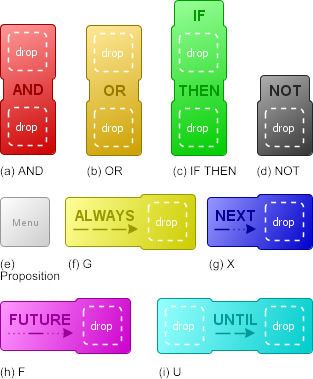
\includegraphics[scale=0.5]{table}
  \caption{The visual language consists of eight unary or binary operator types and one state proposition, each of them having its own color flavor. Logical operators are arranged in a vertical row wereas time relevant statements are aligned horizontally.}
  \label{fig:operators}
\end{figure}



To meet the requirements the visual language should be very easy to use, especially for non-experts. Furthermore it should provide an intuitive application which is ideally learnable within little time. So there are some design decisions an editor for this visual language must fulfill~\cite{moody-physics-of-notations}:

\begin{itemize}
	\item Each operator has a different significant visual appearance; in this case we have used color. This kind of classification enables a faster subconscious identification by the user.
	\item All editing is performed only by simple drag and drop. Operators and propositions can be moved and dropped onto other operators. A tool bar provides all operator and proposition types to be instantiated and there is a trash can for deleting existing operators.
	\item The layout of constraints (nested operators) has two dimensions with a certain meaning. Figure~\ref{fig:directions} demonstrates the ``logical'' vertical read direction as well as the time releveant horizontal line.
	\item In order to simplify the reading of constraints an operator can be hovered over by the mouse pointer. All higher operators become bleached out so that the hovered operator and its children appear highlighted. It's intended to be similar to line coloring when reading a digital text.
	\item Multiple nested operators of the same kind which have no order priorities such as \emph{OR} or \emph{AND} appear unnecessarily complex. These operators can be merged as shown in figure~\ref{fig:nested_and}.
	\item Every edit to either the constraint or the underlying state machine results in an automatically (re-)validation of the constraint. The result is immediately displayed to the user.
	\item There is no button for constraint creation / editing except operator and proposition providers, which let the developer create new instances. Having no additional buttons reduces complexity and keeps it simple.
\end{itemize}


\begin{figure}[htbp]
  \centering
  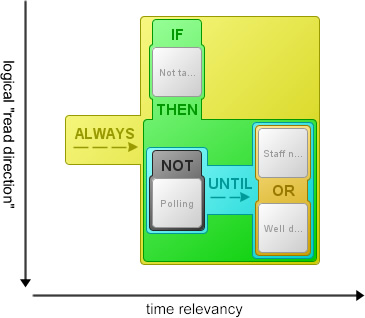
\includegraphics[scale=0.5]{directions}
  \caption{Easy understanding of visual constraints due to intuitive read directions: ``ALWAYS is true: IF state \emph{'Not taken yet'} is active THEN state \emph{'Polling'} can NOT be visited UNTIL state \emph{'Staff notified'} OR state \emph{'Well done!'} is reached.''}
  \label{fig:directions}
\end{figure}

\begin{figure}[htbp]
  \centering
  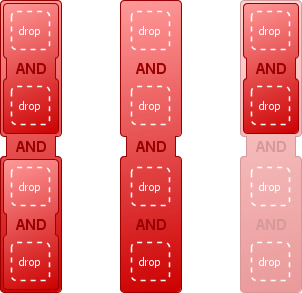
\includegraphics[scale=0.5]{and_simplify} %width=0.7\linewidth
  \caption{In order to simplify the appearance of constraints certain operators might be merged. Merged nested \emph{AND} operators (center) are less complex as default ones (left). However nested \emph{AND} operators with mouse over (right) are displayed separated in order to retain full editability.}
  \label{fig:nested_and}
\end{figure}









\subsection{Automated constraint generation}
\label{sec:automatedconstraintgeneration}

In order to support the developer in specifying safety constraints, automated generation and suggestion of constraints might be helpful. But it's helpful only if the suggested constraints are relevant and reasonable. This however depends on the domain and use case.
Regarding the postulated constraints in the requirements in section~\ref{sec:requirements} all the relevant states have one of the following characteristics:
%following types of states are of a special interest:

\begin{enumerate}
	\item States having two or more outgoing transitions ($\alpha$-states).
	\item States in which all paths starting from one $\alpha$-state come together again ($\beta$-states).
	\item All States immediately before $\beta$ states ($\gamma$-states).
\end{enumerate}

In order to compute the required constraints automatically, and possibly additional ones, we manage a set of subgraphs defined as follows:
%Um die in requirements definierten constraints und vielleicht noch mehr zu finden, behelfen wir uns 
%Each $\alpha$-, the corresponding $\beta$- and several $\gamma$-states form a part of a state set called \emph{subgraph}. In order to retreive valid constraints a subgraph is defined by the following requirements: %as follows

\begin{itemize}
	\item It has a start state ($\alpha$-state) with at least two outgoing transitions.
	\item There is one end state ($\beta$-state) in which all possible paths starting from start state come together again.
	\item All states between the start and end states have no other incoming transitions than the ones originally coming from the start state. That means there is no path to visit these states except through the start state.
	\item The start state may have incoming transitions from states not contained in the subgraph.
	\item The end state may have incoming and outgoing transitions from and to states not contained in the subgraph.
\end{itemize}


\begin{figure}[htbp]
  \centering
  
  \tikzstyle{state} = [circle,fill=white,draw]
  \tikzstyle{statein} = [circle,fill=blue!20,draw]
  \tikzstyle{every path} = [font=\sffamily\small]
  
	\begin{tikzpicture}[->,>=stealth',shorten >=1pt,auto,node distance=15mm]
	
	  \node[statein] (1) {$\alpha$};
	  \node[state] (2) [above left of=1] {};
	  \node[state] (3) [above right of=1] {};
	  \node[statein] (4) [below left of=1] {};
	  \node[statein] (6) [below of=4] {$\gamma$};
	  \node[statein] (7) [below right of=4] {$\gamma$};
	  \node[statein] (5) [below right of=1] {};
	  \node[statein] (8) [below of=5] {$\gamma$};
	  \node[statein] (9) [below of=7] {$\beta$};
	  \node[state] (10) [right of=9] {};
	  \node[state] (11) [below left of=9] {};
	  \node[state] (12) [below right of=9] {};
	  
	  \path[dashed]
	    (2) edge node [left] {} (1)
	    (3) edge node [left] {} (1)
	    (10) edge node [left] {} (9)
	    (9) edge node [left] {} (11)
	    (9) edge node [left] {} (12);
		\path[]
	  	(1) edge node [left] {} (4)
	        edge node [left] {} (5)
	    (4) edge node [left] {} (6)
	        edge node [left] {} (7)
	    (5) edge node [left] {} (8)
	    (6) edge node [left] {} (9)
	    (7) edge node [left] {} (9)
	    (8) edge node [left] {} (9)
	    ;
	
	\end{tikzpicture}
  \caption{Example for a subgraph.}
  \label{fig:subgraph}
\end{figure}

Using this specification all possible such subgraphs can be detected within a state machine. If the subgraph contains neither inner (infinite) loops nor final states (states having no outgoing transition) we can derive the following valid LTL formulas for each subgraph (with $\alpha$ as proposition for ``$\alpha$ is current state'' and similarily for $\beta$ and all $\gamma$'s):

\begin{equation} \label{eq:first}
  \models G (\alpha \Rightarrow F \beta)
\end{equation}

\begin{equation} \label{eq:second}
  \models G (\alpha \Rightarrow F (\bigvee_{\gamma} \gamma))
\end{equation}

\begin{equation} \label{eq:third}
  \models G (\alpha \Rightarrow [\neg \beta U \bigvee_{\gamma} \gamma])
\end{equation}

Additionaly for all states not contained in the subgraph (let's call them $\delta$-states, and the proposition $\delta$ stands for ``$\delta$ is current state'') the following formula is true: 

\begin{equation} \label{eq:fourth}
  \models G (\alpha \Rightarrow [(\bigwedge_{\delta} \neg \delta) U \beta])
\end{equation}

In case of $\alpha = \beta$ -- i.e. when all paths starting from $\alpha$-state eventually return again (cycle) -- even one more constraint can be assumed to be true:

\begin{equation} \label{eq:fifth}
  \models G F \alpha
\end{equation}
 

These five constraints apply for each subgraph matching the conditions mentioned above. Formula~\ref{eq:first} says that an $\alpha$-state is always eventually followed by a $\beta$-state. Formula~\ref{eq:second} ensures that there will be always at least one $\gamma$-state be visited after each visit of an $\alpha$-state. The quite similar but stricter formula~\ref{eq:third} demands additionally a visit of at least one $\gamma$-state before the $\beta$-state can be reached. Formula~\ref{eq:fourth} simply says that a state not contained in the subgraph can't be visited between $\alpha$- and $\beta$-states. That the $\alpha$-state will always eventually be visited again is expressed by formula~\ref{eq:fifth}.

All formulas can be translated to the visual formalism presented in section~\ref{sec:visualformalism} and shown to the user. The appropriate LTL formulas for the postulated constraints in section~\ref{sec:requirements} belong to number \ref{eq:second} and \ref{eq:fifth} of the subgraph based formula templates and are as follows:

\begin{equation}
  \models G F \textnormal{'Polling'}
\end{equation}

\begin{equation}
	\models G (\textnormal{'Not taken yet'} \Rightarrow F (\textnormal{'Well done!'} \vee \textnormal{'Staff notified'})
\end{equation}
%	\item The program will always eventually check the database for new reminder jobs. Thus we avoid that pending reminder are never processed.
%	\item Either a reminded medication is taken properly or caregivers get notified whenever a patient refuses medication intake.


%----------------------------------------------------------------------
% SECTION III: Prototype and evaluation
%----------------------------------------------------------------------
\section{Prototype and evaluation}

To explore and evaluate the visual formalism as well as the usefulness of constraint generation we developed an editor which provides all proposed functionality while taking the requirements into account.
The implementation is a java swing component, making it easy to integrate the visual language into other java applications. An API enables an underlying state machine which also influences the state propositions available for constraint editing. Furthermore a particular model checker can be specified for constraint validation. As a default, the symbolic model checker NuSMV~\cite{springerlink:10.1007/s100090050046,NuSMV2} is used.

Figure~\ref{fig:editor} shows a snapshot of the editor's environment: All functionality needed for constraint editing is provided in the tool bar on the right which contains drag providers for the creating of all operator and proposition types as well as a trashcan for deleting. Constraints can be composed in the dashboard in the middle of the editor by drag and drop. The tab functionality on the left allows several constraints to be managed. Each tab shows a small thumbnail of the constraint and a symbol indicating its validity, which is a warning shield for ``incomplete'', a green shield for ``valid'', a red cross for ``invalid'' or an animated ring for ``validation in progress.'' The magic wand button within the tab pane triggers the constraint generation.

\begin{figure}[htbp]
  \centering
  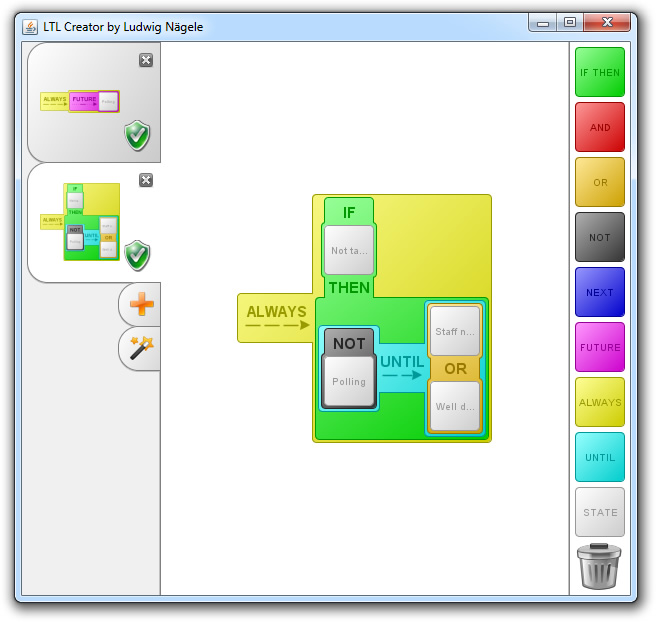
\includegraphics[width=\linewidth]{editor} 
  \caption{Snapshot of the visual editor.}
  \label{fig:editor}
\end{figure}

In order to evaluate the proposed safety functionality the tool was integrated into Robostudio~\cite{robostudio}. It allows the specification of state machine based programs whose behaviour can then be examined by visual constraints. As an example we consider the simplified medication reminder application whose underlying screen-flow is explained in figure~\ref{fig:medicationreminder}. Starting from ``Menu'' the user can choose from several services such as blood pressure measurement or entertainment. In the given example these services are simplified to just one state ``additional services'' since we want to focus only on the medication reminder part. In ``Polling'' the database is checked for a pending reminder, and if there is one the medication intake guidance is triggered. The patient can state if he or she has already taken the medication, or decide whether to take it or not. In the latter he or she may give a reason for it and a caregiver is notified about this incident. Otherwise it will result in ``Well done!'' after completing intake.

\begin{figure}[htbp]
  \centering
  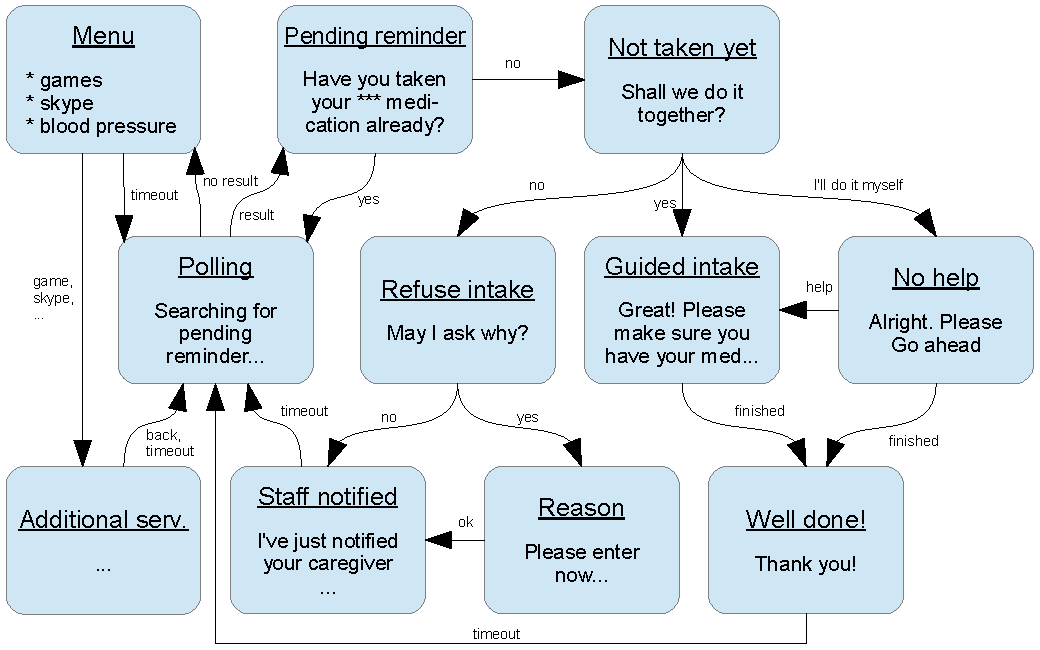
\includegraphics[width=\linewidth]{stm.pdf} %width=0.7\linewidth
  \caption{Simplified screen-flow of the medication reminder application.
  % ** COMMENT: THIS ONE IS TOO SMALL! SHOULD MAKE IT BIGGER TO MAKE TEXT READABLE **
  }
  \label{fig:medicationreminder}
\end{figure}





\subsection{Visual constraints}

Before we can start creating constraints it might be useful to think about a reasonable term we want to express. Let's take the example ``Either a reminded medication is taken properly or caregivers get notified whenever a patient refuses medication intake'' given in the requirements in section~\ref{sec:requirements}.

In order to find a corresponding graphical constraint the sentence has to be modified a little bit so that it fits the underlying state machine: ``Whenever there is a pending reminder, medication will be finally taken or caregivers will get notified in case of refuse''.
Since ``whenever'' is a semantic equivalent to ``always if'' first of all a \emph{GLOBALLY} operator gets dragged to the dashboard directly followed by an \emph{IF} as shown in figure~\ref{fig:sampleconstraint}. The condition for this \emph{IF} is that there is a pending reminder, so a state ``Not taken yet'' has to be added to the upper bucket of the \emph{IF} operator.
Whenever the just mentioned condition becomes true, there also has to be true in future: Medication is taken properly or caregivers get notified about refuse. Accordingly a \emph{FUTURE} operator containing an \emph{OR} forms the second part of the \emph{IF} operator. Finally two states 'Well done!' and 'Staff notified' get added to the disjunction. The resulting visual constraint can now be translated to the corresponding LTL formula by the editor:

\begin{equation} \label{eq:sampleconstraint}
  \models G (\textnormal{'Not taken yet'} \Rightarrow F (\textnormal{'Well done!'} \vee \textnormal{'Staff notified'}))
\end{equation}

%This expression can now be translated to the visual form as we just have to break down the formula from the outside to the inside. A surrounding \emph{GLOBALLY} encapsulates an \emph{IF} block since it is the substitution for \emph{IMPLIES}. Its first operator is a proposition \emph{'Not taken yet'} whereas the second parameter has to be a \emph{FOLLOWS} block containing a disjunction of two propositions \emph{'Well done!'} and \emph{'Staff notified'}. The resulting visual constraint is shown in figure~\ref{fig:sampleconstraint}.

\begin{figure}[htbp]
  \centering
  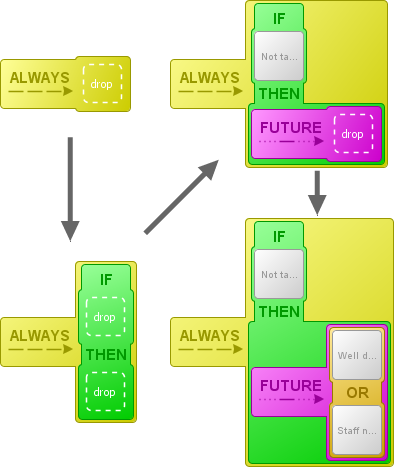
\includegraphics[scale=0.5]{sampleconstraint}
  \caption{Visual constraint creation for LTL formula ~\ref{eq:sampleconstraint}.}
  \label{fig:sampleconstraint}
\end{figure}

After each change within the dashboard the constraint is automatically recompiled and revalidated by using the underlying model checker. As long as the constraint is not completed an ``incomplete'' sign is displayed in the regarding tab. Otherwise an animated ring indicates validation in progress what finally results in either a ``valid'' or ``invalid'' sign.

\begin{figure}[htbp]
  \centering
  
\includegraphics[scale=0.5]{results}
  \caption{Status indicators displayed during or after validation: incomplete, validation in progress, invalid and valid.}
  \label{fig:results}
\end{figure}

NuSMV performs well so even the validation of constraints on huge and complex programs is fast and allows rapid feedback. In addition, the validation itself runs in the background without locking the dashboard. Therefore we have removed waiting times and disruptions during constraint development, which would be likely with conventional model checking where constraint development and constraint validation are alternating processes. Thus we consider our tools an improvement for the users' experience.


\subsection{Constraint generation}
\label{sec:prototypeandevaluation_constraintgeneration}

The automated constraint generation can be triggered by a click on the magic wand button in the tab area. After activation a dashboard is opened in a new tab for each found constraint, and validation is initiated immediately. For the medication reminder application six constraints are found, including \emph{a)} and \emph{b)} shown in figure~\ref{fig:generatedconstraints} which match the postulations in the requirements in section~\ref{sec:requirements}.
The constraint used for demonstration in the previous section is also generated, however \emph{b)} forms an intensified restriction of it.

Constraint \emph{a)} ensures the ``Polling'' state is always eventually visited again. If a pending medication is not already taken, constraint \emph{b)} guarantees intake or staff notification before the next reminders can be read from the database.

We showed that the subgraph approach is working for the medication reminder application, and there was even one more reasonable constraint found by the heuristic: Constraint \emph{c)} ensures that during the medication intake process the program can not switch back to the menu or other services such as entertainment or blood pressure measurement.

%** COMMENT: Possible comment here about the scalability and practicality about constraint generation; do you think it will explode in larger cases? Either way a comment might be useful. **

\begin{figure}[htbp]
  \centering
  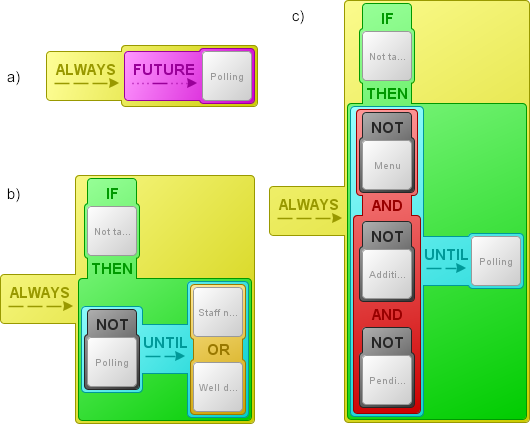
\includegraphics[width=\linewidth]{generatedconstraints} %width=0.7\linewidth
  \caption{Automatically generated constraints which match the postulations in the requirements.}
  \label{fig:generatedconstraints}
\end{figure}



%Da der subgraph-finde-algorithmus als brute force algorithmus implementiert wurde kann bei gro�en programmen (ab ca. 1000 Zust�nden und sehr vielen Verzweigungen) der findeprozess teils sehr lange (mehrere Minuten) dauern. Um den warteprozess ertr�glicher zu machen wird w�hrend der findung ein dialog mit dem aktuellen fortschritt und einem abbrechen button angezeigt.
% hat uns die automatische generierung geholfen? Wuhu, wir haben noch einen constraint gefunden, der auch sinn macht



%----------------------------------------------------------------------
% SECTION III: Prototype and evaluation
%----------------------------------------------------------------------
\section{Future work}

The editor presented in this paper proves validity of all constraints and presents the result \emph{valid} or \emph{invalid} to the user. But in contrast to conventional model checking no additional explanation for the outcome such as a counter example is given. It can be considered to extend the visual language with support for bug identification by a visualization of counter examples, for example.
%\item Substitution of parts of constraints would be nice in order to make it easier to understand. (A simple operator which abstracts from a more complex operator). It's comparable to composite states of hirachical state machines.

%\item A feature which can display an counter example in case a constraint is not valid. It would make the user comprehend the reason in what situation a constraint fails.

%	\item constraints bewerten (nach gewichtung?) und nur wichtige vorschlagen? Oder zumindest sortieren


Since we focus on the healthcare domain in this paper the only proposition type for constraint creation is the state proposition. But to suit other domains additional proposition types such as number or string equations might be added. Also the portability of the constraint generation heuristic to other domains should be examined and different methods than subgraph based constraint finding might be elaborated.


A more systematic evaluation of the tool is required, however this is beyond the scope of the current project. Now that a visual language and tool have been proposed, the next step is to evaluate the tool on a number of applications, make any required modications, then evaluate the tool in a user study for healthcare robotic applications. 	

%\begin{itemize}
%	\item As already mentioned
%	\item Yet, there are only states and no variable expressions etc.
%	\item Substitution of parts of constraints would be nice in order to make it easier to understand. (A simple operator which abstracts from a more complex operator). It's comparable to composite states of hirachical state machines.
%	\item A feature which can display an counter example in case a constraint is not valid. It would make the user comprehend the reason in what situation a constraint fails.
%	\item Problem mit der Zustandsbenennung! Die Zust�nde m�ssen passende Namen haben, was aber nicht immer m�glich ist. Daher m�sste man eigentlich auch Transitionsbedingungen in den Constraints erlauben
%	\item constraints bewerten (nach gewichtung?) und nur wichtige vorschlagen? Oder zumindest sortieren
% \item es wird nur gutes gefunden (also was passieren muss). es werden keine constraints gefunden, die schlechte abl�ufe darstellenund verbieten
%	\item �bertragbarkeit auf andere dom�nen untersuchen?
%	\item A bigger generation algorithm. As already metioned our approach only targets the healthcare domain. Especially the constraint generation can be improved to match also other domains. vielleicht geht beim triggern der constraint generierung ein fenster auf, wo man die heuristic angeben kann (eventuell benannt und gegliedert nach domains).
%\end{itemize}


















% An example of a floating figure using the graphicx package.
% Note that \label must occur AFTER (or within) \caption.
% For figures, \caption should occur after the \includegraphics.
% Note that IEEEtran v1.7 and later has special internal code that
% is designed to preserve the operation of \label within \caption
% even when the captionsoff option is in effect. However, because
% of issues like this, it may be the safest practice to put all your
% \label just after \caption rather than within \caption{}.
%
% Reminder: the "draftcls" or "draftclsnofoot", not "draft", class
% option should be used if it is desired that the figures are to be
% displayed while in draft mode.
%
%\begin{figure}[!t]
%\centering
%\includegraphics[width=2.5in]{myfigure}
% where an .eps filename suffix will be assumed under latex, 
% and a .pdf suffix will be assumed for pdflatex; or what has been declared
% via \DeclareGraphicsExtensions.
%\caption{Simulation Results}
%\label{fig_sim}
%\end{figure}

% Note that IEEE typically puts floats only at the top, even when this
% results in a large percentage of a column being occupied by floats.


% An example of a double column floating figure using two subfigures.
% (The subfig.sty package must be loaded for this to work.)
% The subfigure \label commands are set within each subfloat command, the
% \label for the overall figure must come after \caption.
% \hfil must be used as a separator to get equal spacing.
% The subfigure.sty package works much the same way, except \subfigure is
% used instead of \subfloat.
%
%\begin{figure*}[!t]
%\centerline{\subfloat[Case I]\includegraphics[width=2.5in]{subfigcase1}%
%\label{fig_first_case}}
%\hfil
%\subfloat[Case II]{\includegraphics[width=2.5in]{subfigcase2}%
%\label{fig_second_case}}}
%\caption{Simulation results}
%\label{fig_sim}
%\end{figure*}
%
% Note that often IEEE papers with subfigures do not employ subfigure
% captions (using the optional argument to \subfloat), but instead will
% reference/describe all of them (a), (b), etc., within the main caption.


% An example of a floating table. Note that, for IEEE style tables, the 
% \caption command should come BEFORE the table. Table text will default to
% \footnotesize as IEEE normally uses this smaller font for tables.
% The \label must come after \caption as always.
%
%\begin{table}[!t]
%% increase table row spacing, adjust to taste
%\renewcommand{\arraystretch}{1.3}
% if using array.sty, it might be a good idea to tweak the value of
% \extrarowheight as needed to properly center the text within the cells
%\caption{An Example of a Table}
%\label{table_example}
%\centering
%% Some packages, such as MDW tools, offer better commands for making tables
%% than the plain LaTeX2e tabular which is used here.
%\begin{tabular}{|c||c|}
%\hline
%One & Two\\
%\hline
%Three & Four\\
%\hline
%\end{tabular}
%\end{table}


% Note that IEEE does not put floats in the very first column - or typically
% anywhere on the first page for that matter. Also, in-text middle ("here")
% positioning is not used. Most IEEE journals/conferences use top floats
% exclusively. Note that, LaTeX2e, unlike IEEE journals/conferences, places
% footnotes above bottom floats. This can be corrected via the \fnbelowfloat
% command of the stfloats package.



\section{Conclusion}

In this paper we represented a visual formalism for the defining of safety constraints and a concept of automated constraint generation. Both features are implemented and assembled in an editor for standalone or integrated use. The visual language is reasonably simple which makes it accessible to a wider range of software developers. Nevertheless it is reasonably expressive and allows serious model checking.

The concept of constraint generation worked very well for our use case, the medication reminder application, and all postulated constraints were found. Since we even discovered a new reasonable constraint we are convinced this concept as well as the visual language for defining constraints has the potential to support development of safety critical healthcare robot applications.




% conference papers do not normally have an appendix


% use section* for acknowledgement
\section*{Acknowledgment}

This work evolved from a master thesis project provided by the Elite Graduate Program Software Engineering. 
For the received support the authors would like to thank the people of this program and the three patron universities: University of Augsburg, Technical University Munich and Ludwig-Maximilians-University Munich.
 
%The authors would like to thank for support received from the  which is held by the tree universities .





% trigger a \newpage just before the given reference
% number - used to balance the columns on the last page
% adjust value as needed - may need to be readjusted if
% the document is modified later
%\IEEEtriggeratref{8}
% The "triggered" command can be changed if desired:
%\IEEEtriggercmd{\enlargethispage{-5in}}

% references section

% can use a bibliography generated by BibTeX as a .bbl file
% BibTeX documentation can be easily obtained at:
% http://www.ctan.org/tex-archive/biblio/bibtex/contrib/doc/
% The IEEEtran BibTeX style support page is at:
% http://www.michaelshell.org/tex/ieeetran/bibtex/
\bibliographystyle{IEEEtran}
% argument is your BibTeX string definitions and bibliography database(s)
\bibliography{IEEEabrv,Paper}
%
% <OR> manually copy in the resultant .bbl file
% set second argument of \begin to the number of references
% (used to reserve space for the reference number labels box)
%\begin{thebibliography}{1}
%\bibitem{healthcare}
%B.~MacDonald, \emph{Healthcare}.
%\bibitem{robostudio}
%C.~Datta and B.~MacDonald, \emph{Robostudio}.

%\bibitem{visualtemporallogic1993}
%\emph{1993 A Visual-Programming Environment for a Temporal Logic Language}.
%\bibitem{visualtemporallogic1995}
%\emph{1995 Visual Specification of Branching Time Temporal Logic}.
%\bibitem{hometl}
%\emph{2007 HomeTL: A visual formalism, based on temporal logic, for the design of home based care}.
%\bibitem{adl}
%\emph{2007 A Visual Editor to Support the Use of Temporal Logic for ADL Monitoring}.


%\bibitem{IEEEhowto:kopka}
%H.~Kopka and P.~W. Daly, \emph{A Guide to \LaTeX}, 3rd~ed.\hskip 1em plus
%  0.5em minus 0.4em\relax Harlow, England: Addison-Wesley, 1999.

%\end{thebibliography}




% that's all folks
\end{document}


